\documentclass{article}
\usepackage{MyPack2}
\usepackage{pgfplots}
\usepackage[justification=centering]{caption}
\usepackage{placeins}

\newcommand{\resultat}[2]{
  \begin{figure}[!htb]
  \centering
  \input{../../generationDeGraph/resultats/#1}
  \caption{#2}
  \label{#1}
  \end{figure}
}
\renewcommand{\topfraction}{.75}
\renewcommand{\bottomfraction}{.75}

\title{TIPE : Propagation de rumeurs dans un réseau social\\Rapport}
\author{Hugo LEVY-FALK}
\date{2017}

\begin{document}
\maketitle
\initPage{TIPE 2017}{Propagation de rumeurs}{Hugo LEVY-FALK}\;
\tableofcontents
\newpage

\section{Préambule}
Ce rapport synthétise le travail réalisé sur la propagation de rumeurs dans les réseaux sociaux. On cherche à propager le plus efficacement possible une rumeur à l'ensemble d'un réseau. Les objectifs fixés lors de la mise en cohérence ont étés atteints.

\section{Introduction}
Faisant suite à la recherche documentaire, une première approche théorique de la propagation des rumeurs, s'inspirant du livre de Easley et Kleinberg, a été réalisée. Cela permet de fixer le cadre des simulations ainsi que d'identifier les paramètres des expériences. Dans un deuxième temps trois critères de choix des propagateurs initiaux ont été expérimentés en faisant varier les paramètres mis en évidence précédemment.

\section{Propagation de rumeurs}
\subsection{Modalités d'action}
\subsubsection{Étude théorique}
L'étude théorique a consisté en la formalisation des concepts de rumeur et de propagation. On modélise naturellement un réseau social par un graphe $G = (V,E)$, avec $V$ un ensemble de nœuds et $E\subset V²$, que l'on supposera connexe par la suite. Chaque membre du réseau est modélisé par un nœud du graphe et ses liens sociaux par des arrêtes.

On cherche d'abord à caractériser le comportement d'un nœud. Pour cela on considère qu'un nœud peut se trouver dans deux états distincts : il transmet la rumeur à tous ses voisins ($A$) ou il ne relaie pas la rumeur ($B$). Pour chaque nœud $i\in V$, si $i$ est dans l'état $A$, alors pour chacun des ses voisins également dans l'état $A$, $i$ réalise un gain $a$. De même si $i$ est dans l'état $B$, il réalise un gain $b$ pour chacun de ses voisins dans l'état $B$. On procède ensuite à une simulation où, à chaque étape, tous les nœuds du graphe tentent de maximiser leur gain en choisissant ou non de passer à l'état $A$ (on n'autorise pas les passages de $A$ vers $B$).

Lors d'une étape de simulation, si l'on note $p$ la proportion de voisins dans l'état $A$ du nœud $i$, alors le nœud $i$ maximise son gain en passant à l'état $A$ si $p \times a > (1-p) \times b$, ou encore $$ p > \frac{b}{a+b} = q$$ 

\begin{prop}
  \label{impossible1}
  Si $q > 1$, alors la rumeur ne peut pas se propager.
\end{prop}

\begin{prop}
  \label{stationnaire}
  Si l'on pose $(V_k)_{k\in\N}$ la suite des nœuds dans l'état $A$ à l'étape $k$, s'il existe $n\in\N$ tel que $V_n = V_{n+1}$ alors la suite est stationnaire à partir du rang n.
\end{prop}
\begin{proof}
  Si $V_n = V_{n+1}$ alors chaque nœud maximise déjà son gain à l'étape $n$, la situation étant identique à l'étape $n+1$, on a $V_{n+1} = V_{n+2}$.
\end{proof}

Dans la suite on pose $n=|V|$.

\begin{prop}
  \label{convergente}
  La suite $(V_k)_{k\in\N}$ converge en $n$ étapes au plus.
\end{prop}
\begin{proof}
  La suite $(V_k)_{k\in\N}$ étant croissante pour l'inclusion et majorée par $V$, elle converge. D'autre part, d'après la proposition \ref{stationnaire}, elle est stationnaire à partir du rang $k\in\N$ si $V_k = V_{k+1}$. Or il n'y a que $n$ nœuds, donc la suite est stationnaire à partir du rang $n-1$ au plus. 
\end{proof}

La proposition \ref{convergente} assure que toutes les simulations pourront être terminées en un temps fini. La proposition \ref{stationnaire} permet de raccourcir la durée d'une simulation en comptant le nombre d'éléments qui passent à l'état $A$ à chaque étape de simulation. S'il est nul, alors la simulation est terminée.

On cherche ensuite un critère plus complet que la proposition \ref{impossible1} pour qualifier la possibilité de propager une rumeur.
\begin{defi}
  On appelle $p$-cluster tout $C \subset V$ tel que pour $i\in C$ il existe $(v_k)_{k\in \llbracket1,p\rrbracket} \in C^p$ deux à deux distincts et tels que pour tout $k\in \llbracket1,p\rrbracket$, $i$ et $v_k$ soient voisins.
\end{defi}

\begin{theo}
  Une rumeur de note $q$ ne se propagera pas à l'ensemble du réseau si et seulement si il existe un $p$-cluster non initialement informé avec $p>q$.
\end{theo}
\begin{proof}
  S'il existe un $p$-cluster C avec $p>q$, alors tout nœud de C possède au moins une proportion $p$ de voisins non informés. Ceci valant pour tous les nœuds de C, aucun nœud de C ne sera informé au bout de $n$ étapes. \emph{Les clusters sont des obstacles aux rumeurs.}

  S'il existe un nœud $i\in V$ tel qu'au bout de $n$ étapes $i$ ne soit pas dans l'état informé, alors la proportion $p$ de voisins de $i$ dans l'état informé vérifie $p \leq q$ ou encore $(1-p) > q \leq 0$. Il existe donc des voisins de $i$ vérifiant cette propriété, \emph{on a un $z$-cluster avec $z>q$}.
\end{proof}

\subsubsection{Génération des graphes}

Les graphes sont générés avec l'algorithme de Watts-Strogatz qui permet de générer des graphes connexes vérifiant le phénomène du "petit monde" mis en évidence par Milgram.

\begin{algorithm}[H]
\Donnees{$N \in \N, K \in \llbracket 1, \lfloor\frac{N}{2}\rfloor\rrbracket (N \gg K \gg \ln N), \beta \in [0,1]$
}
\Res{Matrice d'adjacence d'un graphe aléatoire.}
$M \leftarrow $ matrice avec pour $i\in \llbracket0,N-1\rrbracket$, $j\in \llbracket1,K\rrbracket$, $M_{i,i+j[N]} = M_{i,i-j[N]} = \text{Vrai}$, Faux pour les autres \;
\Pour{$i\in \llbracket0,N-1\rrbracket$}{
  \Pour{$j\in \llbracket1,K\rrbracket$}{
    $r \leftarrow$ Nombre aléatoire sur $[0,1]$\;
    \Si{$r<\beta$}{
      $M_{i,i+j[N]} \leftarrow $ Faux\;
      $M_{i+j[N],i} \leftarrow $ Faux\;
      Choisir au hasard $k$ tel que $M_{i,k}=\text{Faux}$\;
      $M_{i,k} \leftarrow $ Vrai\;
      $M_{k,i} \leftarrow $ Vrai\;
    }
  }
}
\Retour{$M$}
\caption{Algorithme de Watts-Strogatz}
\end{algorithm}

Pour les expériences on fixera $N=500$ et $K=50$. On fera varier $\beta$ dans $\{0,0.25,0.5,0.75,1\}$. L'algorithme a été implémenté en OCaml.

\subsubsection{Expériences}
Il est difficile de définir ce qui est attendu d'une propagation optimale d'une rumeur. On comparera donc trois méthodes de choix des propagateurs initiaux.
\begin{itemize}
  \item Le tirage au sort, à des fins de comparaison;
  \item Les éléments de plus grand degré. En effet une première analyse qualitative laisse penser que ces nœuds seront plus à même de "convaincre" une grande partie du réseau;
  \item Les éléments les plus centraux, c'est à dire ceux par lesquels passent la plus grande proportion de plus courts chemins. Pour cela on utilise l'algorithme de Ulrik Brandes. Cela caractérise la capacité d'un nœud à atteindre rapidement les autres nœuds du graphe.
\end{itemize}

Pour mesurer la capacité de propagation moyenne d'une méthode de choix, on réalise $100$ fois chaque expériences. Étant donné la longueur des calculs, un système de sauvegarde de l'avancement d'une expérience dans une base de données a été implémenté. Ceci permet d'interrompre une expérience et de la reprendre au même endroit lorsque le programme est relancé.

\subsection{Résultats}
On représente les résultats sous la forme d'une courbe $\text{proportion finale}=f(\text{proportion initiale})$. La courbe type obtenue est décrite à la figure \ref{random_finale_f_initiale_q50_Beta50_ec}.

\resultat{random_finale_f_initiale_q50_Beta50_ec}{Courbe type (en pointillés rouge l'écart type)}

Le paramètre $\beta$ a essentiellement une influence dans le choix par centralité. Les résultats sont résumés dans les figures \ref{resultats1}, \ref{resultats2} et \ref{resultats3}.
\begin{figure}
\centering
% This file was created by matplotlib2tikz v0.6.7.
\begin{tikzpicture}

\definecolor{color0}{rgb}{0.75,0,0.75}

\begin{axis}[
title={Taille du graphe:500 Échantillon:100 K=50, q=$\frac{1}{4}$},
xlabel={Proportion initiale},
ylabel={Proportion finale},
xmin=-0.039, xmax=1.039,
ymin=-0.0395, ymax=1.0495,
width=\textwidth,
height=.33\textheight,
tick align=outside,
tick pos=left,
xmajorgrids,
x grid style={lightgray!92.026143790849673!black},
ymajorgrids,
y grid style={lightgray!92.026143790849673!black},
legend cell align={left},
legend style={at={(0.97,0.03)}, anchor=south east, draw=white!80.0!black},
legend entries={{Identité},{Degré},{Aléatoire},{Centralité $\beta=\frac{1}{4}$},{Centralité $\beta=\frac{3}{4}$}}
]
\addplot [line width=1.0pt, lightgray!66.928104575163388!black, dashed]
table {%
0.01 0.01
0.02 0.02
0.03 0.03
0.04 0.04
0.05 0.05
0.06 0.06
0.07 0.07
0.08 0.08
0.09 0.09
0.1 0.1
0.11 0.11
0.12 0.12
0.13 0.13
0.14 0.14
0.15 0.15
0.16 0.16
0.17 0.17
0.18 0.18
0.19 0.19
0.2 0.2
0.21 0.21
0.22 0.22
0.23 0.23
0.24 0.24
0.25 0.25
0.26 0.26
0.27 0.27
0.28 0.28
0.29 0.29
0.3 0.3
0.31 0.31
0.32 0.32
0.33 0.33
0.34 0.34
0.35 0.35
0.36 0.36
0.37 0.37
0.38 0.38
0.39 0.39
0.4 0.4
0.41 0.41
0.42 0.42
0.43 0.43
0.44 0.44
0.45 0.45
0.46 0.46
0.47 0.47
0.48 0.48
0.49 0.49
0.5 0.5
0.51 0.51
0.52 0.52
0.53 0.53
0.54 0.54
0.55 0.55
0.56 0.56
0.57 0.57
0.58 0.58
0.59 0.59
0.6 0.6
0.61 0.61
0.62 0.62
0.63 0.63
0.64 0.64
0.65 0.65
0.66 0.66
0.67 0.67
0.68 0.68
0.69 0.69
0.7 0.7
0.71 0.71
0.72 0.72
0.73 0.73
0.74 0.74
0.75 0.75
0.76 0.76
0.77 0.77
0.78 0.78
0.79 0.79
0.8 0.8
0.81 0.81
0.82 0.82
0.83 0.83
0.84 0.84
0.85 0.85
0.86 0.86
0.87 0.87
0.88 0.88
0.89 0.89
0.9 0.9
0.91 0.91
0.92 0.92
0.93 0.93
0.94 0.94
0.95 0.95
0.96 0.96
0.97 0.97
0.98 0.98
0.99 0.99
};
\addplot [line width=1.0pt, red]
table {%
0.01 0.01
0.02 0.02
0.03 0.03
0.04 0.04
0.05 0.0499999999999999
0.06 0.0599999999999999
0.07 0.0700600000000001
0.08 0.08948
0.09 0.1091
0.1 0.2187
0.11 0.46892
0.12 0.88626
0.13 0.99132
0.14 1
0.15 1
0.16 1
0.17 1
0.18 1
0.19 1
0.2 1
0.21 1
0.22 1
0.23 1
0.24 1
0.25 1
0.26 1
0.27 1
0.28 1
0.29 1
0.3 1
0.31 1
0.32 1
0.33 1
0.34 1
0.35 1
0.36 1
0.37 1
0.38 1
0.39 1
0.4 1
0.41 1
0.42 1
0.43 1
0.44 1
0.45 1
0.46 1
0.47 1
0.48 1
0.49 1
0.5 1
0.51 1
0.52 1
0.53 1
0.54 1
0.55 1
0.56 1
0.57 1
0.58 1
0.59 1
0.6 1
0.61 1
0.62 1
0.63 1
0.64 1
0.65 1
0.66 1
0.67 1
0.68 1
0.69 1
0.7 1
0.71 1
0.72 1
0.73 1
0.74 1
0.75 1
0.76 1
0.77 1
0.78 1
0.79 1
0.8 1
0.81 1
0.82 1
0.83 1
0.84 1
0.85 1
0.86 1
0.87 1
0.88 1
0.89 1
0.9 1
0.91 1
0.92 1
0.93 1
0.94 1
0.95 1
0.96 1
0.97 1
0.98 1
0.99 1
};
\addplot [line width=1.0pt, green!50.196078431372548!black]
table {%
0.01 0.012
0.02 0.022
0.03 0.032
0.04 0.0419999999999999
0.05 0.0519999999999999
0.06 0.0620000000000001
0.07 0.07202
0.08 0.0820199999999999
0.09 0.09228
0.1 0.12074
0.11 0.17574
0.12 0.34358
0.13 0.70668
0.14 0.949
0.15 1
0.16 1
0.17 1
0.18 1
0.19 1
0.2 1
0.21 1
0.22 1
0.23 1
0.24 1
0.25 1
0.26 1
0.27 1
0.28 1
0.29 1
0.3 1
0.31 1
0.32 1
0.33 1
0.34 1
0.35 1
0.36 1
0.37 1
0.38 1
0.39 1
0.4 1
0.41 1
0.42 1
0.43 1
0.44 1
0.45 1
0.46 1
0.47 1
0.48 1
0.49 1
0.5 1
0.51 1
0.52 1
0.53 1
0.54 1
0.55 1
0.56 1
0.57 1
0.58 1
0.59 1
0.6 1
0.61 1
0.62 1
0.63 1
0.64 1
0.65 1
0.66 1
0.67 1
0.68 1
0.69 1
0.7 1
0.71 1
0.72 1
0.73 1
0.74 1
0.75 1
0.76 1
0.77 1
0.78 1
0.79 1
0.8 1
0.81 1
0.82 1
0.83 1
0.84 1
0.85 1
0.86 1
0.87 1
0.88 1
0.89 1
0.9 1
0.91 1
0.92 1
0.93 1
0.94 1
0.95 1
0.96 1
0.97 1
0.98 1
0.99 1
};
\addplot [line width=1.0pt, color0]
table {%
0.01 0.01
0.02 0.02
0.03 0.9709
0.04 1
0.05 1
0.06 1
0.07 1
0.08 1
0.09 1
0.1 1
0.11 1
0.12 1
0.13 1
0.14 1
0.15 1
0.16 1
0.17 1
0.18 1
0.19 1
0.2 1
0.21 1
0.22 1
0.23 1
0.24 1
0.25 1
0.26 1
0.27 1
0.28 1
0.29 1
0.3 1
0.31 1
0.32 1
0.33 1
0.34 1
0.35 1
0.36 1
0.37 1
0.38 1
0.39 1
0.4 1
0.41 1
0.42 1
0.43 1
0.44 1
0.45 1
0.46 1
0.47 1
0.48 1
0.49 1
0.5 1
0.51 1
0.52 1
0.53 1
0.54 1
0.55 1
0.56 1
0.57 1
0.58 1
0.59 1
0.6 1
0.61 1
0.62 1
0.63 1
0.64 1
0.65 1
0.66 1
0.67 1
0.68 1
0.69 1
0.7 1
0.71 1
0.72 1
0.73 1
0.74 1
0.75 1
0.76 1
0.77 1
0.78 1
0.79 1
0.8 1
0.81 1
0.82 1
0.83 1
0.84 1
0.85 1
0.86 1
0.87 1
0.88 1
0.89 1
0.9 1
0.91 1
0.92 1
0.93 1
0.94 1
0.95 1
0.96 1
0.97 1
0.98 1
0.99 1
};
\addplot [line width=1.0pt, blue]
table {%
0.01 0.01
0.02 0.02
0.03 0.03
0.04 0.04
0.05 0.0500799999999999
0.06 0.0602399999999999
0.07 0.0707400000000001
0.08 0.08322
0.09 0.12596
0.1 0.54828
0.11 0.95648
0.12 1
0.13 1
0.14 1
0.15 1
0.16 1
0.17 1
0.18 1
0.19 1
0.2 1
0.21 1
0.22 1
0.23 1
0.24 1
0.25 1
0.26 1
0.27 1
0.28 1
0.29 1
0.3 1
0.31 1
0.32 1
0.33 1
0.34 1
0.35 1
0.36 1
0.37 1
0.38 1
0.39 1
0.4 1
0.41 1
0.42 1
0.43 1
0.44 1
0.45 1
0.46 1
0.47 1
0.48 1
0.49 1
0.5 1
0.51 1
0.52 1
0.53 1
0.54 1
0.55 1
0.56 1
0.57 1
0.58 1
0.59 1
0.6 1
0.61 1
0.62 1
0.63 1
0.64 1
0.65 1
0.66 1
0.67 1
0.68 1
0.69 1
0.7 1
0.71 1
0.72 1
0.73 1
0.74 1
0.75 1
0.76 1
0.77 1
0.78 1
0.79 1
0.8 1
0.81 1
0.82 1
0.83 1
0.84 1
0.85 1
0.86 1
0.87 1
0.88 1
0.89 1
0.9 1
0.91 1
0.92 1
0.93 1
0.94 1
0.95 1
0.96 1
0.97 1
0.98 1
0.99 1
};
\end{axis}

\end{tikzpicture}
\caption{Résultats}
\label{resultats1}
\end{figure}
\begin{figure}
\centering
% This file was created by matplotlib2tikz v0.6.7.
\begin{tikzpicture}

\definecolor{color0}{rgb}{0.75,0,0.75}

\begin{axis}[
title={Taille du graphe:500 Échantillon:100 K=50, q=$\frac{1}{2}$},
xlabel={Proportion initiale},
ylabel={Proportion finale},
xmin=-0.039, xmax=1.039,
ymin=-0.0395, ymax=1.0495,
width=\textwidth,
height=.33\textheight,
tick align=outside,
tick pos=left,
xmajorgrids,
x grid style={lightgray!92.026143790849673!black},
ymajorgrids,
y grid style={lightgray!92.026143790849673!black},
legend cell align={left},
legend style={at={(0.97,0.03)}, anchor=south east, draw=white!80.0!black},
legend entries={{Identité},{Degré},{Aléatoire},{Centralité $\beta=\frac{1}{4}$},{Centralité $\beta=\frac{3}{4}$}}
]
\addplot [line width=1.0pt, lightgray!66.928104575163388!black, dashed]
table {%
0.01 0.01
0.02 0.02
0.03 0.03
0.04 0.04
0.05 0.05
0.06 0.06
0.07 0.07
0.08 0.08
0.09 0.09
0.1 0.1
0.11 0.11
0.12 0.12
0.13 0.13
0.14 0.14
0.15 0.15
0.16 0.16
0.17 0.17
0.18 0.18
0.19 0.19
0.2 0.2
0.21 0.21
0.22 0.22
0.23 0.23
0.24 0.24
0.25 0.25
0.26 0.26
0.27 0.27
0.28 0.28
0.29 0.29
0.3 0.3
0.31 0.31
0.32 0.32
0.33 0.33
0.34 0.34
0.35 0.35
0.36 0.36
0.37 0.37
0.38 0.38
0.39 0.39
0.4 0.4
0.41 0.41
0.42 0.42
0.43 0.43
0.44 0.44
0.45 0.45
0.46 0.46
0.47 0.47
0.48 0.48
0.49 0.49
0.5 0.5
0.51 0.51
0.52 0.52
0.53 0.53
0.54 0.54
0.55 0.55
0.56 0.56
0.57 0.57
0.58 0.58
0.59 0.59
0.6 0.6
0.61 0.61
0.62 0.62
0.63 0.63
0.64 0.64
0.65 0.65
0.66 0.66
0.67 0.67
0.68 0.68
0.69 0.69
0.7 0.7
0.71 0.71
0.72 0.72
0.73 0.73
0.74 0.74
0.75 0.75
0.76 0.76
0.77 0.77
0.78 0.78
0.79 0.79
0.8 0.8
0.81 0.81
0.82 0.82
0.83 0.83
0.84 0.84
0.85 0.85
0.86 0.86
0.87 0.87
0.88 0.88
0.89 0.89
0.9 0.9
0.91 0.91
0.92 0.92
0.93 0.93
0.94 0.94
0.95 0.95
0.96 0.96
0.97 0.97
0.98 0.98
0.99 0.99
};
\addplot [line width=1.0pt, red]
table {%
0.01 0.01
0.02 0.02
0.03 0.03
0.04 0.04
0.05 0.0499999999999999
0.06 0.0599999999999999
0.07 0.0700000000000001
0.08 0.0800000000000001
0.09 0.0899999999999999
0.1 0.0999999999999998
0.11 0.11
0.12 0.12
0.13 0.13
0.14 0.14
0.15 0.15
0.16 0.16
0.17 0.17
0.18 0.18
0.19 0.19002
0.2 0.20002
0.21 0.21
0.22 0.22002
0.23 0.23008
0.24 0.24014
0.25 0.25022
0.26 0.2606
0.27 0.27816
0.28 0.28134
0.29 0.2934
0.3 0.30588
0.31 0.46044
0.32 0.59948
0.33 0.81028
0.34 0.94918
0.35 1
0.36 1
0.37 1
0.38 1
0.39 1
0.4 1
0.41 1
0.42 1
0.43 1
0.44 1
0.45 1
0.46 1
0.47 1
0.48 1
0.49 1
0.5 1
0.51 1
0.52 1
0.53 1
0.54 1
0.55 1
0.56 1
0.57 1
0.58 1
0.59 1
0.6 1
0.61 1
0.62 1
0.63 1
0.64 1
0.65 1
0.66 1
0.67 1
0.68 1
0.69 1
0.7 1
0.71 1
0.72 1
0.73 1
0.74 1
0.75 1
0.76 1
0.77 1
0.78 1
0.79 1
0.8 1
0.81 1
0.82 1
0.83 1
0.84 1
0.85 1
0.86 1
0.87 1
0.88 1
0.89 1
0.9 1
0.91 1
0.92 1
0.93 1
0.94 1
0.95 1
0.96 1
0.97 1
0.98 1
0.99 1
};
\addplot [line width=1.0pt, green!50.196078431372548!black]
table {%
0.01 0.012
0.02 0.022
0.03 0.032
0.04 0.0419999999999999
0.05 0.0519999999999999
0.06 0.0620000000000001
0.07 0.0720000000000001
0.08 0.0819999999999999
0.09 0.0919999999999999
0.1 0.102
0.11 0.112
0.12 0.122
0.13 0.132
0.14 0.142
0.15 0.152
0.16 0.162
0.17 0.172
0.18 0.182
0.19 0.192
0.2 0.202
0.21 0.212
0.22 0.222
0.23 0.23202
0.24 0.242000000000001
0.25 0.25202
0.26 0.26202
0.27 0.27206
0.28 0.28228
0.29 0.292180000000001
0.3 0.30266
0.31 0.31292
0.32 0.32418
0.33 0.33552
0.34 0.37446
0.35 0.47698
0.36 0.65582
0.37 0.8282
0.38 0.97612
0.39 1
0.4 1
0.41 1
0.42 1
0.43 1
0.44 1
0.45 1
0.46 1
0.47 1
0.48 1
0.49 1
0.5 1
0.51 1
0.52 1
0.53 1
0.54 1
0.55 1
0.56 1
0.57 1
0.58 1
0.59 1
0.6 1
0.61 1
0.62 1
0.63 1
0.64 1
0.65 1
0.66 1
0.67 1
0.68 1
0.69 1
0.7 1
0.71 1
0.72 1
0.73 1
0.74 1
0.75 1
0.76 1
0.77 1
0.78 1
0.79 1
0.8 1
0.81 1
0.82 1
0.83 1
0.84 1
0.85 1
0.86 1
0.87 1
0.88 1
0.89 1
0.9 1
0.91 1
0.92 1
0.93 1
0.94 1
0.95 1
0.96 1
0.97 1
0.98 1
0.99 1
};
\addplot [line width=1.0pt, color0]
table {%
0.01 0.01
0.02 0.02
0.03 0.03
0.04 0.04
0.05 0.0499999999999999
0.06 0.0605399999999999
0.07 0.0752
0.08 0.09512
0.09 0.11206
0.1 0.13032
0.11 0.14554
0.12 0.15962
0.13 0.1752
0.14 0.19346
0.15 0.20622
0.16 0.2247
0.17 0.2367
0.18 0.24808
0.19 0.2619
0.2 0.27692
0.21 0.29258
0.22 0.30928
0.23 0.31494
0.24 0.33046
0.25 0.34438
0.26 0.36026
0.27 0.37378
0.28 0.38378
0.29 0.40162
0.3 0.40992
0.31 0.4222
0.32 0.43942
0.33 0.44724
0.34 0.46026
0.35 0.49936
0.36 0.51134
0.37 0.52054
0.38 0.5412
0.39 0.57592
0.4 0.6489
0.41 0.67108
0.42 0.7399
0.43 0.77416
0.44 0.81748
0.45 0.85282
0.46 0.9245
0.47 0.91522
0.48 0.93398
0.49 0.95978
0.5 0.98206
0.51 0.99312
0.52 0.99316
0.53 1
0.54 0.9965
0.55 1
0.56 1
0.57 0.9963
0.58 0.99642
0.59 1
0.6 1
0.61 1
0.62 1
0.63 1
0.64 1
0.65 1
0.66 1
0.67 1
0.68 1
0.69 1
0.7 1
0.71 1
0.72 1
0.73 1
0.74 1
0.75 1
0.76 1
0.77 1
0.78 1
0.79 1
0.8 1
0.81 1
0.82 1
0.83 1
0.84 1
0.85 1
0.86 1
0.87 1
0.88 1
0.89 1
0.9 1
0.91 1
0.92 1
0.93 1
0.94 1
0.95 1
0.96 1
0.97 1
0.98 1
0.99 1
};
\addplot [line width=1.0pt, blue]
table {%
0.01 0.01
0.02 0.02
0.03 0.03
0.04 0.04
0.05 0.0499999999999999
0.06 0.0599999999999999
0.07 0.0700000000000001
0.08 0.0800000000000001
0.09 0.0899999999999999
0.1 0.0999999999999998
0.11 0.11
0.12 0.12
0.13 0.13
0.14 0.14
0.15 0.15
0.16 0.16008
0.17 0.17
0.18 0.18002
0.19 0.19012
0.2 0.20014
0.21 0.21036
0.22 0.22054
0.23 0.23114
0.24 0.2418
0.25 0.25248
0.26 0.26402
0.27 0.27502
0.28 0.28756
0.29 0.29946
0.3 0.31368
0.31 0.33012
0.32 0.35382
0.33 0.3641
0.34 0.43798
0.35 0.6088
0.36 0.78154
0.37 0.9558
0.38 0.97772
0.39 0.99462
0.4 1
0.41 1
0.42 1
0.43 1
0.44 1
0.45 1
0.46 1
0.47 1
0.48 1
0.49 1
0.5 1
0.51 1
0.52 1
0.53 1
0.54 1
0.55 1
0.56 1
0.57 1
0.58 1
0.59 1
0.6 1
0.61 1
0.62 1
0.63 1
0.64 1
0.65 1
0.66 1
0.67 1
0.68 1
0.69 1
0.7 1
0.71 1
0.72 1
0.73 1
0.74 1
0.75 1
0.76 1
0.77 1
0.78 1
0.79 1
0.8 1
0.81 1
0.82 1
0.83 1
0.84 1
0.85 1
0.86 1
0.87 1
0.88 1
0.89 1
0.9 1
0.91 1
0.92 1
0.93 1
0.94 1
0.95 1
0.96 1
0.97 1
0.98 1
0.99 1
};
\end{axis}

\end{tikzpicture}
\caption{Résultats}
\label{resultats2}
\end{figure}
\begin{figure}
\centering
% This file was created by matplotlib2tikz v0.6.7.
\begin{tikzpicture}

\definecolor{color0}{rgb}{0.75,0,0.75}

\begin{axis}[
title={Taille du graphe:500 Échantillon:100 K=50, q=$\frac{3}{4}$},
xlabel={Proportion initiale},
ylabel={Proportion finale},
xmin=-0.039, xmax=1.039,
ymin=-0.0395, ymax=1.0495,
width=\textwidth,
height=.33\textheight,
tick align=outside,
tick pos=left,
xmajorgrids,
x grid style={lightgray!92.026143790849673!black},
ymajorgrids,
y grid style={lightgray!92.026143790849673!black},
legend cell align={left},
legend style={at={(0.97,0.03)}, anchor=south east, draw=white!80.0!black},
legend entries={{Identité},{Degré},{Aléatoire},{Centralité $\beta=\frac{1}{4}$},{Centralité $\beta=\frac{3}{4}$}}
]
\addplot [line width=1.0pt, lightgray!66.928104575163388!black, dashed]
table {%
0.01 0.01
0.02 0.02
0.03 0.03
0.04 0.04
0.05 0.05
0.06 0.06
0.07 0.07
0.08 0.08
0.09 0.09
0.1 0.1
0.11 0.11
0.12 0.12
0.13 0.13
0.14 0.14
0.15 0.15
0.16 0.16
0.17 0.17
0.18 0.18
0.19 0.19
0.2 0.2
0.21 0.21
0.22 0.22
0.23 0.23
0.24 0.24
0.25 0.25
0.26 0.26
0.27 0.27
0.28 0.28
0.29 0.29
0.3 0.3
0.31 0.31
0.32 0.32
0.33 0.33
0.34 0.34
0.35 0.35
0.36 0.36
0.37 0.37
0.38 0.38
0.39 0.39
0.4 0.4
0.41 0.41
0.42 0.42
0.43 0.43
0.44 0.44
0.45 0.45
0.46 0.46
0.47 0.47
0.48 0.48
0.49 0.49
0.5 0.5
0.51 0.51
0.52 0.52
0.53 0.53
0.54 0.54
0.55 0.55
0.56 0.56
0.57 0.57
0.58 0.58
0.59 0.59
0.6 0.6
0.61 0.61
0.62 0.62
0.63 0.63
0.64 0.64
0.65 0.65
0.66 0.66
0.67 0.67
0.68 0.68
0.69 0.69
0.7 0.7
0.71 0.71
0.72 0.72
0.73 0.73
0.74 0.74
0.75 0.75
0.76 0.76
0.77 0.77
0.78 0.78
0.79 0.79
0.8 0.8
0.81 0.81
0.82 0.82
0.83 0.83
0.84 0.84
0.85 0.85
0.86 0.86
0.87 0.87
0.88 0.88
0.89 0.89
0.9 0.9
0.91 0.91
0.92 0.92
0.93 0.93
0.94 0.94
0.95 0.95
0.96 0.96
0.97 0.97
0.98 0.98
0.99 0.99
};
\addplot [line width=1.0pt, red]
table {%
0.01 0.01
0.02 0.02
0.03 0.03
0.04 0.04
0.05 0.0499999999999999
0.06 0.0599999999999999
0.07 0.0700000000000001
0.08 0.0800000000000001
0.09 0.0899999999999999
0.1 0.0999999999999998
0.11 0.11
0.12 0.12
0.13 0.13
0.14 0.14
0.15 0.15
0.16 0.16
0.17 0.17
0.18 0.18
0.19 0.19
0.2 0.2
0.21 0.21
0.22 0.22
0.23 0.23
0.24 0.24
0.25 0.25
0.26 0.260000000000001
0.27 0.27
0.28 0.28
0.29 0.289999999999999
0.3 0.3
0.31 0.309999999999999
0.32 0.32
0.33 0.329999999999999
0.34 0.34
0.35 0.350000000000001
0.36 0.36
0.37 0.37
0.38 0.38
0.39 0.39
0.4 0.399999999999999
0.41 0.409999999999999
0.42 0.420000000000001
0.43 0.43
0.44 0.44
0.45 0.45004
0.46 0.460100000000001
0.47 0.470079999999999
0.48 0.480279999999999
0.49 0.49024
0.5 0.50066
0.51 0.51098
0.52 0.52106
0.53 0.53184
0.54 0.54292
0.55 0.55414
0.56 0.56716
0.57 0.57992
0.58 0.59952
0.59 0.63432
0.6 0.72444
0.61 0.863
0.62 0.95208
0.63 0.99372
0.64 1
0.65 1
0.66 1
0.67 1
0.68 1
0.69 1
0.7 1
0.71 1
0.72 1
0.73 1
0.74 1
0.75 1
0.76 1
0.77 1
0.78 1
0.79 1
0.8 1
0.81 1
0.82 1
0.83 1
0.84 1
0.85 1
0.86 1
0.87 1
0.88 1
0.89 1
0.9 1
0.91 1
0.92 1
0.93 1
0.94 1
0.95 1
0.96 1
0.97 1
0.98 1
0.99 1
};
\addplot [line width=1.0pt, green!50.196078431372548!black]
table {%
0.01 0.012
0.02 0.022
0.03 0.032
0.04 0.0419999999999999
0.05 0.0519999999999999
0.06 0.0620000000000001
0.07 0.0720000000000001
0.08 0.0819999999999999
0.09 0.0919999999999999
0.1 0.102
0.11 0.112
0.12 0.122
0.13 0.132
0.14 0.142
0.15 0.152
0.16 0.162
0.17 0.172
0.18 0.182
0.19 0.192
0.2 0.202
0.21 0.212
0.22 0.222
0.23 0.232
0.24 0.242000000000001
0.25 0.252
0.26 0.262
0.27 0.272
0.28 0.282
0.29 0.292000000000001
0.3 0.302
0.31 0.312
0.32 0.321999999999999
0.33 0.332000000000001
0.34 0.341999999999999
0.35 0.352
0.36 0.362
0.37 0.372
0.38 0.382
0.39 0.392
0.4 0.402
0.41 0.412
0.42 0.422
0.43 0.432
0.44 0.442
0.45 0.452
0.46 0.462000000000001
0.47 0.472000000000001
0.48 0.481999999999999
0.49 0.492079999999999
0.5 0.502000000000001
0.51 0.51208
0.52 0.522159999999999
0.53 0.532139999999999
0.54 0.542520000000001
0.55 0.55272
0.56 0.562959999999999
0.57 0.57372
0.58 0.58406
0.59 0.59566
0.6 0.6072
0.61 0.62048
0.62 0.63456
0.63 0.68722
0.64 0.74854
0.65 0.92058
0.66 0.99122
0.67 1
0.68 1
0.69 1
0.7 1
0.71 1
0.72 1
0.73 1
0.74 1
0.75 1
0.76 1
0.77 1
0.78 1
0.79 1
0.8 1
0.81 1
0.82 1
0.83 1
0.84 1
0.85 1
0.86 1
0.87 1
0.88 1
0.89 1
0.9 1
0.91 1
0.92 1
0.93 1
0.94 1
0.95 1
0.96 1
0.97 1
0.98 1
0.99 1
};
\addplot [line width=1.0pt, color0]
table {%
0.01 0.01
0.02 0.02
0.03 0.03
0.04 0.04
0.05 0.0499999999999999
0.06 0.0599999999999999
0.07 0.0700000000000001
0.08 0.0800000000000001
0.09 0.0899999999999999
0.1 0.10002
0.11 0.11
0.12 0.12022
0.13 0.1303
0.14 0.14096
0.15 0.15148
0.16 0.16182
0.17 0.1727
0.18 0.18318
0.19 0.19384
0.2 0.20526
0.21 0.21664
0.22 0.22716
0.23 0.23784
0.24 0.2499
0.25 0.25974
0.26 0.27102
0.27 0.28134
0.28 0.29128
0.29 0.30388
0.3 0.31368
0.31 0.32464
0.32 0.3347
0.33 0.34504
0.34 0.35606
0.35 0.3664
0.36 0.37712
0.37 0.38774
0.38 0.39728
0.39 0.40826
0.4 0.41886
0.41 0.42902
0.42 0.44038
0.43 0.4488
0.44 0.46026
0.45 0.47022
0.46 0.48224
0.47 0.49078
0.48 0.50256
0.49 0.51176
0.5 0.52096
0.51 0.53264
0.52 0.54234
0.53 0.55238
0.54 0.56266
0.55 0.57146
0.56 0.58222
0.57 0.59486
0.58 0.60316
0.59 0.61316
0.6 0.62372
0.61 0.63328
0.62 0.64282
0.63 0.6537
0.64 0.66246
0.65 0.67296
0.66 0.68292
0.67 0.693360824742268
0.68 0.7024
0.69 0.7125
0.7 0.7229
0.71 0.73258
0.72 0.74244
0.73 0.75276
0.74 0.76212
0.75 0.771100000000001
0.76 0.78034
0.77 0.79034
0.78 0.80078
0.79 0.80984
0.8 0.82054
0.81 0.82998
0.82 0.83966
0.83 0.848619999999999
0.84 0.857839999999999
0.85 0.86756
0.86 0.87706
0.87 0.8846
0.88 0.893000000000001
0.89 0.90192
0.9 0.90852
0.91 0.91604
0.92 0.92416
0.93 0.932140000000001
0.94 0.940519999999999
0.95 0.951480000000001
0.96 0.99414
0.97 1
0.98 1
0.99 1
};
\addplot [line width=1.0pt, blue]
table {%
0.01 0.01
0.02 0.02
0.03 0.03
0.04 0.04
0.05 0.0499999999999999
0.06 0.0599999999999999
0.07 0.0700000000000001
0.08 0.0800000000000001
0.09 0.0899999999999999
0.1 0.0999999999999998
0.11 0.11
0.12 0.12
0.13 0.13
0.14 0.14
0.15 0.15
0.16 0.16
0.17 0.17
0.18 0.18
0.19 0.19
0.2 0.2
0.21 0.21
0.22 0.22
0.23 0.23
0.24 0.24
0.25 0.25
0.26 0.260000000000001
0.27 0.27
0.28 0.28
0.29 0.289999999999999
0.3 0.3
0.31 0.309999999999999
0.32 0.32
0.33 0.329999999999999
0.34 0.34
0.35 0.350000000000001
0.36 0.36
0.37 0.37
0.38 0.38
0.39 0.39002
0.4 0.400019999999999
0.41 0.410039999999999
0.42 0.420060000000001
0.43 0.43004
0.44 0.44008
0.45 0.450200000000001
0.46 0.460340000000001
0.47 0.47038
0.48 0.480479999999999
0.49 0.4905
0.5 0.50082
0.51 0.5108
0.52 0.52104
0.53 0.5315
0.54 0.54206
0.55 0.552
0.56 0.5627
0.57 0.57356
0.58 0.58374
0.59 0.59484
0.6 0.6056
0.61 0.6166
0.62 0.62758
0.63 0.63888
0.64 0.64932
0.65 0.66052
0.66 0.67146
0.67 0.68308
0.68 0.69792
0.69 0.70876
0.7 0.72056
0.71 0.73548
0.72 0.74854
0.73 0.76382
0.74 0.78974
0.75 0.834040000000001
0.76 0.90076
0.77 0.96468
0.78 0.9932
0.79 0.99342
0.8 1
0.81 1
0.82 1
0.83 1
0.84 1
0.85 1
0.86 1
0.87 1
0.88 1
0.89 1
0.9 1
0.91 1
0.92 1
0.93 1
0.94 1
0.95 1
0.96 1
0.97 1
0.98 1
0.99 1
};
\end{axis}

\end{tikzpicture}
\caption{Résultats}
\label{resultats3}
\end{figure}

\FloatBarrier
\subsection{Analyse, exploitation et discussion}
Les résultats montrent que pour des rumeurs relativement convaincantes, c'est-à-dire $q$ faible (ici $<25\%$), le choix par centralité est plus intéressant. En effet pour $\beta = \frac{1}{4}$, une proportion initiale de $5 \%$ des plus centraux permet d'atteindre tout le graphe là où il faut $10 \%$ des éléments de plus hauts degrés.

En revanche, pour des rumeurs avec $q$ élevé ($>50\%$), la méthode des plus hauts degrés est à privilégier. 

Les résultats devraient être confirmés par une étude sur un échantillon plus important de graphes. De plus, les graphes produits par l'algorithme sont irréalistes de par le degré des nœuds et le paramètre $\beta$ dont il est difficile de mesurer l'influence.

Une étude plus précise prenant en compte le caractère cinétique de la propagation (nombre d'étapes pour atteindre tous les nœuds) serait nécessaire pour la tranche $\frac{1}{4} < q < \frac{1}{2}$.

\section{Conclusion}
Cette étude met en évidence une stratégie de choix des éléments propagateurs initiaux, bien que les résultats obtenus demandent une étude complémentaire qui n'a pas été réalisée du fait de la longueur des calculs (l'étude actuelle a déjà nécessité plusieurs centaines d'heures de simulation). Lorsque la rumeur est convaincante, il est préférable de choisir ces éléments pour leur centralité élevée. Sinon, lorsque la rumeur est moins convaincante, il est plus efficace de choisir les éléments de plus haut degré.


\end{document}
